\documentclass[preprint]{emulateapj}
\input{newcommand_gen.tex}
\shorttitle{shorttitle}
\shortauthors{shortauthors}


%%% packages
\usepackage{graphicx}
\usepackage{amsmath}
\usepackage{xspace}
%\usepackage{array}
\usepackage{lineno}

\newcommand{\myemail}{email@email.com}

\begin{document}
\linenumbers

\title{Spin-orbit misalignment for the long period companion of KOI-368}

\author{First Author\altaffilmark{1} and
Second Author\altaffilmark{2}}

\altaffiltext{1}{Affil2; \email{\myemail}}
\altaffiltext{2}{Affil1}

\begin{abstract}
Abstract
\end{abstract}

\keywords{keywords}

\section{Introduction}
\label{sec:introduction}

%Kepler Obliquity measurement
%\citet{Hirano:2012} 
using the rotation period from the lightcurve and 
then combined with the projected rotation period and stellar radius from 
high-res spectrospcopy, measured the obliquity of 15 KOI systems. 

%\citet{Barnes:2011} 
use the asymmetry in the Kepler transit lightcurve of KOI-13 to measure 
the spin-obital alignment angle. 

\section{Method}
\label{sec:method}

{\bf KOI-368} is assigned as Kepler Object of Interesting in the 
Batalha:2013 
from the Quarter 1-6 data. It has a Kepler Input Catalog entry 6603043. 
The KIC parameters of the star are $T_{\rm eff} = 9034 {\rm K}$,  
$\rm logg=4.133$, and $\rm FeH = -0.028$, indicating it is a hot and 
fast rotating star. 
The transit parameter from Kepler catalog is $P = 110.3216019 day$, 
$R=19.16$\rearth.
We make use of the public Kepler Long Cadence (29.4min) (Q1-Q15) and 
Short Cadence (59.s?) data (Q8-Q9) to study the photometry effect 
predicted by 
%\citet{Barnes:2009}
The long cadence data consist of 11 transit althogether (assigned transit 
number from epoch 0-11, with the 7th missing). The short cadence data 
cover transit 5 and 6. 

For transit fitting, we use the $\rm SAP\_FLUX$, the out of transit 
variations are corrected by the following steps (\ref):

a) removal of bad data points;

b) correction of safe mode and tweaks;

c) a set of cosine functions with minimum period of 1 day. 

d) a 7th order polynomial fit on the out of transit parts. 

For analysis of the rotation period of the star, we use the $\rm PDC\_FLUX$ 
(\ref) (Q1-Q?). 

{\bf TBD: the figure of the lightcurve itself?}

%The gravity darkening model

The gravity darkening model is generatied following 
%\citet{Barnes:2009}
The temperature profile on the stellar surface is determined by the local 
effective gravity.
\begin{equation}
\frac{T}{T_{\rm pole}} \propto (\frac{g_{\rm eff}}{g_{\rm pole}})^{\beta}. 
= F_{f,w} (r,\theta)
\end{equation}
f is the oblation of the star, (definition?), w is the nondimension 
measure of the rotation rate, r and \theta are the normalized the position 
parameters.
The gravity darkening parameter $\beta$ is obtained by xxx. 


% \begin{figure}[h!]
%   \centering
%   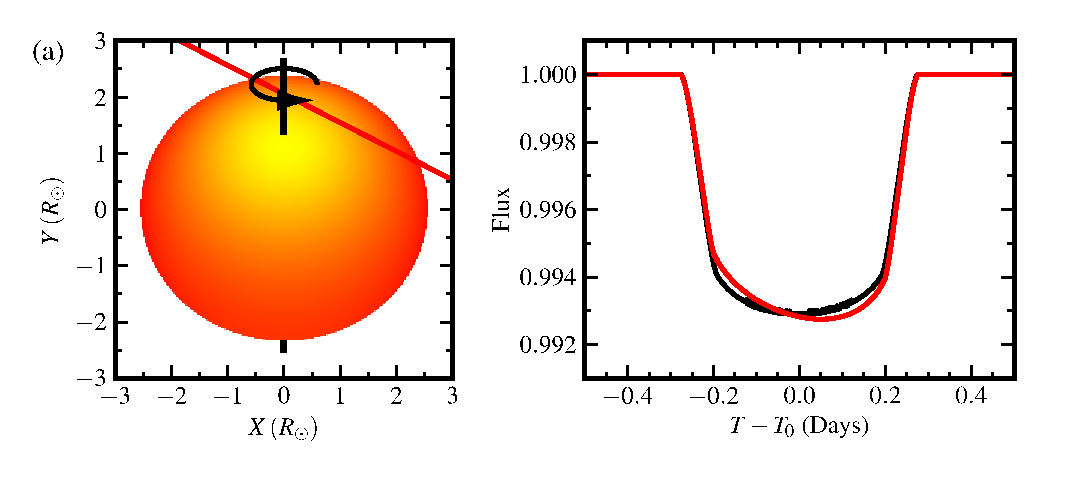
\includegraphics[width=5cm]{obliq_model.eps}
%   \caption{caption}
%   \label{fig:obliq_model}
% \end{figure}
\begin{figure}
  \centering
  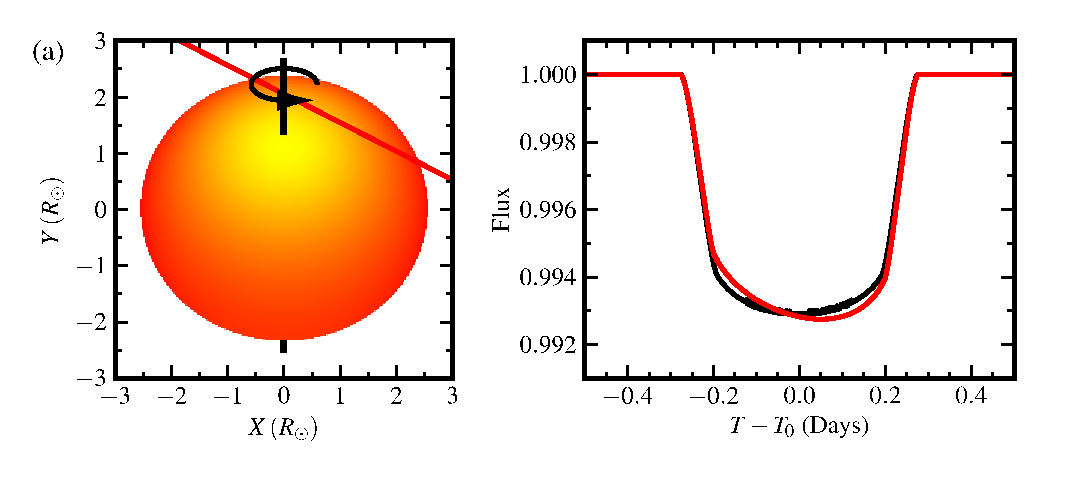
\includegraphics[width=9cm]{obliq_model.eps}
  \caption{caption}
  \label{fig:obliqmodel}
\end{figure}

\subsection{Host star parameters}
\label{sec:host-star-parameters}

[APO observation and spectrum fitting]

We estimate the rotation period of the host star by plotting the
Lomb-Scargle periodogram
\citep[][Figure~\ref{fig:LS}]{1976Ap&amp;SS..39..447L,1982ApJ...263..835S}
for the Kepler PDC long cadence lightcurve, with primary transits masked. The
resulting peaks was checked by the CLEAN algorithm
\citep{1987AJ.....93..968R}. We adopte the first significant peak at 1.19 
days as the rotation period of the host star. [Justify with vsini]

\begin{figure}[h!]
  \centering
  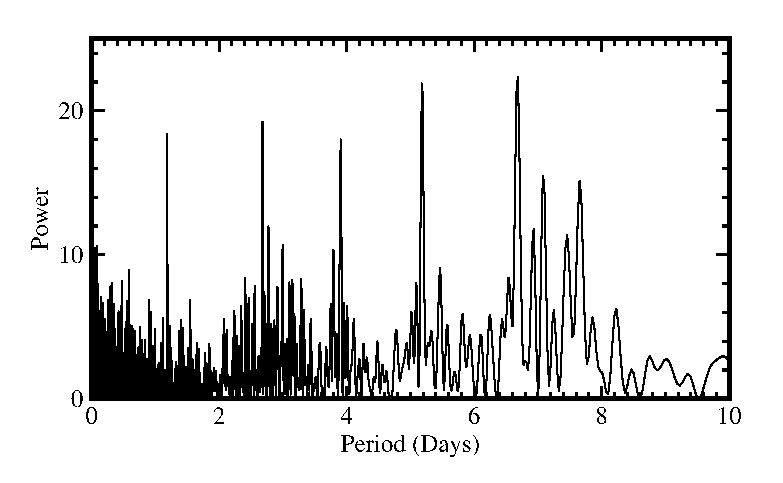
\includegraphics[width=7cm]{LS.eps}
  \caption{Lomb-Scargle periodogram of the PDC lightcurve, with the
    transits masked out. The lightcurve is rotationally modulated with
  a period of 1.19 days.}
  \label{fig:LS}
\end{figure}

\subsection{Transit lightcurve fitting}
\label{sec:transit-light-curve}

The transit lightcurve is modelled using the
\citet{1972ApJ...174..617N} model, implemented in an adaption of the
JKTEBOP code \citep{1981AJ.....86..102P,2004MNRAS.351.1277S}. The
relevant free parameters are orbital period $P$, transit centre $T_0$,
normalised radius sum $R_\star+R_p / a$, radius ratio $R_p/R_\star$,
line of sight inclination $i$, and quadratic limb darkening
coefficients $c_1$ and $c_2$. Initial estimates of the limb darkening
coefficients are taken from \citet{2010A&amp;A...510A..21S}. Jump
parameters for the stellar oblation correction include the planet
orbit obliquity $\lambda$, stellar oblation $f$. The projection angle
between the stellar rotation axis and line of sight $i_\text{rot}$ is
fixed for the initial analysis, then set free to explore the potential
degeneracies. A flux offset for each transit event is calculated and
removed at each iteration, and is not included in the fit
parameters. For Kepler long cadence data, the model is modified by a
30 minute boxcar smooth. The best fit parameters and the posterior
probability distribution is explored via a Markov chain Monte Carlo
(MCMC) analysis, using the \emph{emcee} MCMC ensemble sampler
\citep{2012arXiv1202.3665F}. The likelihood function is given by
$\exp(-\Delta\chi^2/2)$. For each transit, we scale the flux errors such
that the reduced $\chi^2$ is at unity. This allows for errors other
than photon noise to be taken into account.

\begin{figure}[h!]
  \centering
  \includegraphics[width=9cm]{lightcurve.eps}
  \caption{caption}
  \label{fig:lightcurve}
\end{figure}

\section{Analysis}
\label{sec:analysis}

\section{Discussion}
\label{sec:discussion}

\bibliographystyle{apj}
\bibliography{mybibfile}

\end{document}
